\chapter{The informatics of biology}
Bioinformatics is the application of computational methods to biological problems,
either by analysing large amounts of data or by replacing experiments with computer programs.

\section{Predictors}
A significant fraction of the protein bioinformatics work is the development of predictors: statistical or machine learning methods that can, given limited information, predict properties of proteins.
A common choice is to make predictions taking only the amino acid sequence, because this is the easiest information we can acquire of a protein.
Other methods may require extra annotation, such as Gene Ontology -- an annotation condensing all our knowledge of the gene that produced the protein -- or 3D structures -- experimental or models.

\section[Multiple Sequence Alignments]{Increasing statistics: Multiple Sequence Alignments}

\section{Contact prediction}
Folded proteins are tightly packed structures, as illustrated in Figure~\ref{fig:packing}.
Since there is very little to no space between neighbouring residues, not every mutation is allowed.
Proteins that have evolved 


\begin{figure}[!hb]
	\centering
	\hfil
	\subcaptionbox{Cartoon and sticks\label{subfig:sticks}}{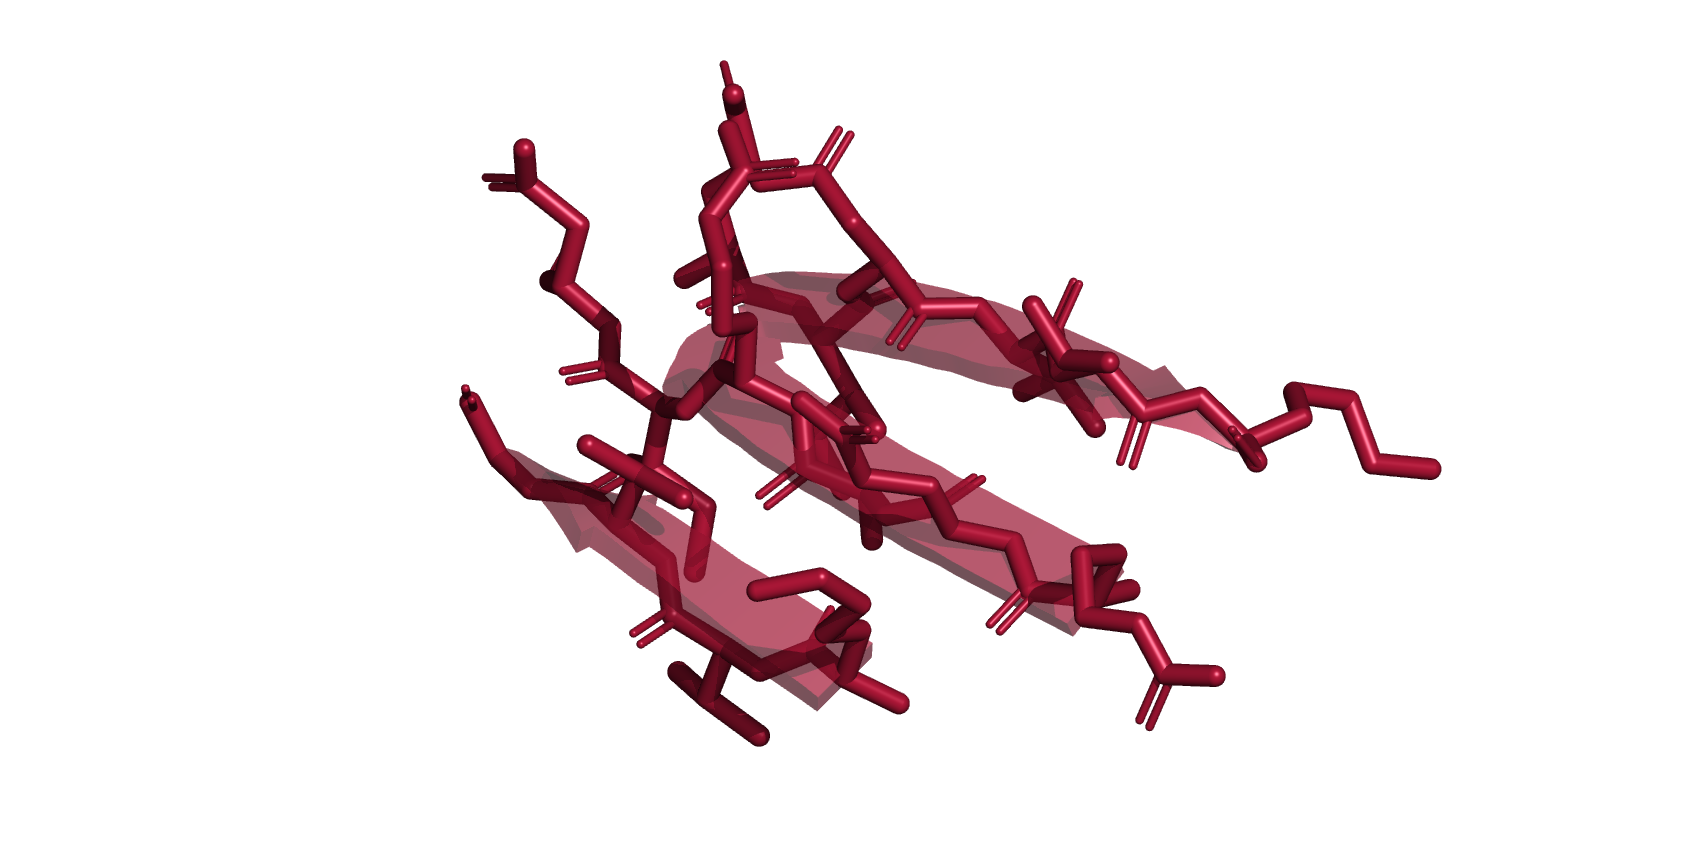
\includegraphics[trim={65mm 3mm 32mm 0},clip, width=0.45\textwidth]{bioinfo/figures/sheet_sticks}}
	\hfil
	\subcaptionbox{Atom-sized spheres\label{subfig:spheres}}{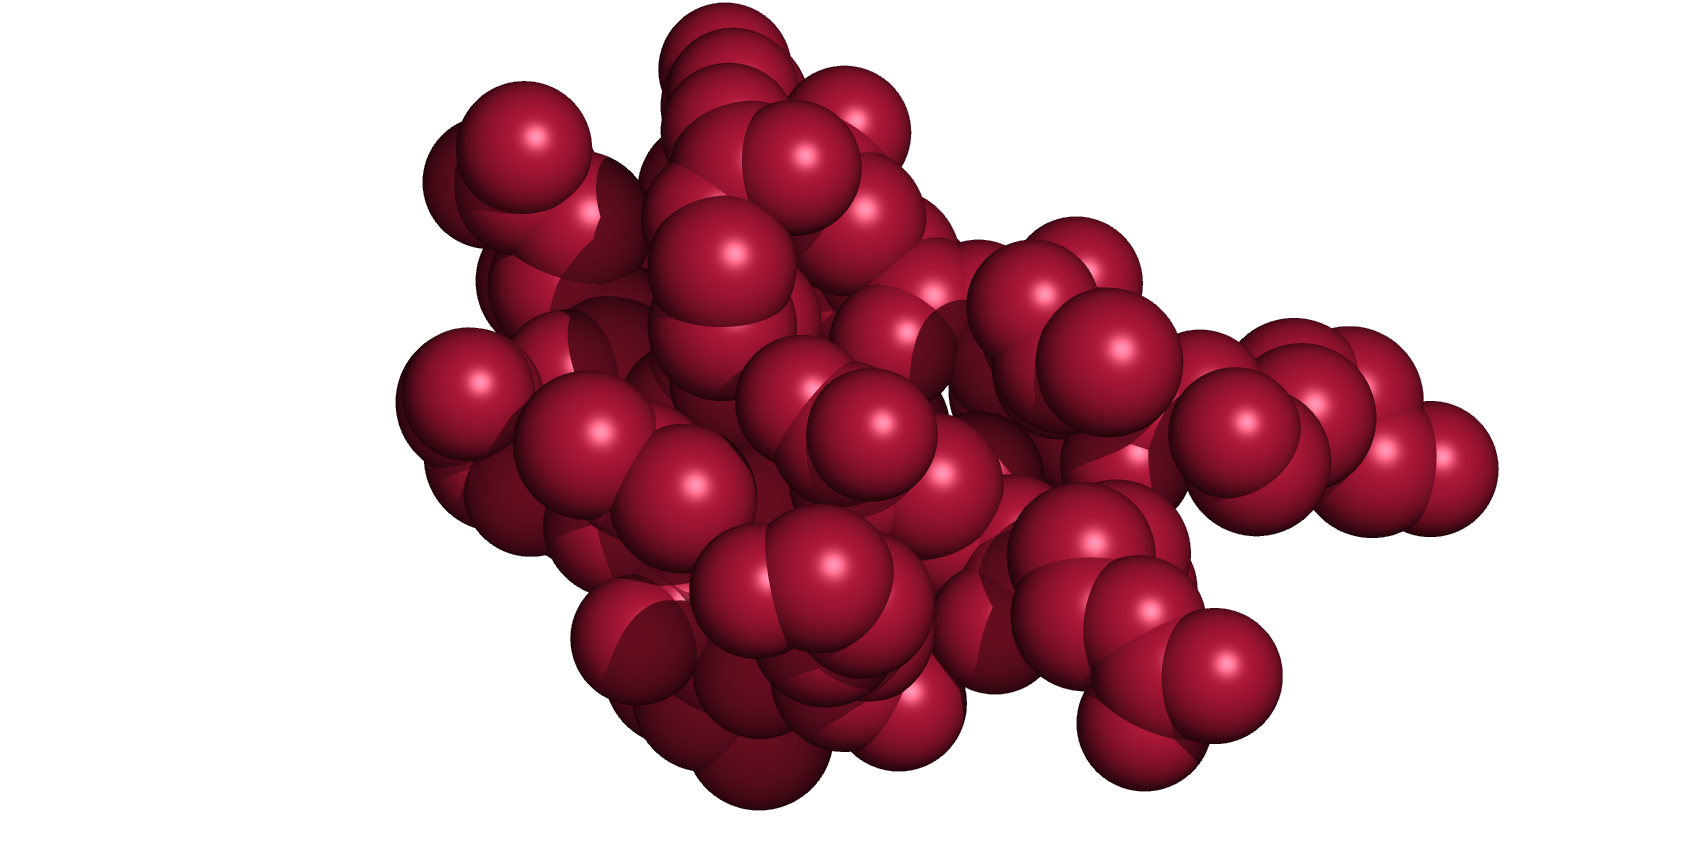
\includegraphics[trim={65mm 3mm 32mm 0},clip, width=0.45\textwidth]{bioinfo/figures/sheet_spheres}}
	\hfil
	\caption{Fragment of a $\beta$-sheet in two representations: cartoon and sticks, and space filling spheres, showing the tightness of the packing.
	They are both seen from the same angle at the same scale.}\label{fig:packing}
\end{figure}

A Multiple Sequence Alignment (MSA) contains a collection of proteins evolutionary related to our query.
\marginpar{Correlated mutations}

\subsection{Mutual Information}

\begin{equation*}
MI\left(i, j\right) = \sum_{x, y}^{q_{max}} f(x_i, y_j) \log \left(\frac{f(x_i, y_j)}{f(x_i)f(y_j)}\right),
\end{equation*}
where $f(x_i, x_j)$ is the joint distribution of amino acids $x_i$ and $y_j$ at positions $i$ and $j$, $f(x_i)$ and $f(y_j)$ are the marginal distributions, and $q_{max}$ is the maximum number of amino acids types in the alignment, including gaps.
If the MSA is of enough quality, the contacts will present high values of $MI$.



\subsection{Direct Coupling Analysis}
Mutual Information has a problem with the transitivity property: consider three residues, A, B, and C; where B is close to both A and C, but A and C are far away.
Mutual Information will likely detect a correlation between A and B, and between B and C; but it will also show a correlation between A and C!

In order to discern true from spurious correlations, we need to fit a statistical model to the whole data at once, in this way, we hope to recover the true (direct) relationships.
This can be accomplished with Direct Coupling Analysis (DCA).
Several variations exist, but they are all based on a Potts model of statistical mechanics.
This is a model where each position (in our case, residue), can take a number of discrete, well-defined, spin states (amino acid types), and the model depends only on the intrinsic properties at each location, and pairwise interactions.

The energy of a sequence of amino acids $\vec{\sigma}$ takes the form:
\begin{equation*}
H(\vec \sigma) = \sum_{\substack{i,j=1\\i \neq j}}^N J_{i, j}(\sigma_i, \sigma_j) + \sum_{i=1}^N h_i(\sigma_i),
\end{equation*}
where $h_i(\sigma_i)$ is the chemical potential of having a given amino acid at position $i$, and $ J_{i, j}(\sigma_i, \sigma_j)$ is the pairwise interaction between residues $i$ and $j$ given their amino acid species.

We can assume the proteins in our MSA were generated by a similar model, so their frequency should follow the Boltzmann distribution:

\begin{equation*}
p(\vec{\sigma} |  h, J) = \frac{1}{Z} e^{-\beta H\left(\vec{\sigma}\right)}
\end{equation*}
$\beta$ is a scaling factor, the inverse of the temperature, and $Z$ is the partition function, a normalisation term to ensure all the probabilities sum up to 1:

\begin{equation*}
Z = \sum_{\vec{\sigma}} e^{-\beta H\left(\vec{\sigma}\right)}
\end{equation*}

Fitting a Potts model means to estimate the values of $J$ and $h$ that best explain the observed distribution of sequences in the MSA.
The problem as such is intractable because computing $Z$ implies a sum over all the possible sequences of length $N$, $21^N$ (the 20 natural amino acids plus the gap state).

There are several strategies that can approximate the partition function, such as plmDCA \citep{plmDCA}, or side-step it all together, like GaussDCA \citep{GaussDCA}.

Once the values of $J$ are obtained, the scores of the contacts can be estimated by taking the Frobenius norm of each of the J matrices.
That is, the square root of the sum of the squares of the couplings between each pair of amino acids:

\begin{equation*}
C(i, j) = \sqrt{\sum_{\sigma_i, \sigma_j=1}^{21} J_{i, j}(\sigma_i, \sigma_j)^2},
\end{equation*}
where $C(i, j)$ is the contact score between residues $i$ and $j$.
This number cannot be readily interpreted as a probability.

This model approximations ignore the possibility of multiple rotamers for a given amino acid \marginpar{The sphericity of the cow}
and consider that any interaction between three or more residues can be decomposed to the sum of each pair.
Finally, DCA attempts to reconstruct the evolutionary couplings, not necessarily the contacts.
\citet{contact_errors} showed that most of the top-scoring pairs indicated by DCA are true contacts, others correspond to contacts between different subunits in a homodimer or pairs of separated residues involved in the function.
The coupling is real, but its nature is different from the model explained at the beginning of this section.

\subsection{Phylogenetic bias: the APC correction}

\subsection{Pattern recognition}
Contacts do not appear at random.
Since the protein is a continuous chain, contacts are rarely isolated, and appear in groups.
Furthermore, since most of the protein is locally organised in secondary structure elements, this gives rise to specific patterns in the contact map.
The statistical methods like DCA and Mutual Information do not consider this, so a refinement step can be done using pattern recognition.
We can train a machine learning algorithm on the outputs of statistical methods and recognise the underlying patterns, which is able to remove much of the spurious contacts, noise, and artefacts in the alignments.

\missingfigure{alpha and beta contacts}

\section{Protein folding}

One of the main goals of protein bioinformatics is predicting the 3D structure of a protein given only its sequence.

\subsection{Physics-based modelling}
Unfolded natural proteins in physiological conditions are known to fold into their native state \citep{fold_graciously}.
In principle, the same procedure can be replicated \emph{in silico} with molecular dynamics, like the work done by \citet{physics_folding}.
This was possible because the domain is very short -- 35 residues --, and fast folding; but in general is not a practical solution, as it requires a lot of computational work.

\subsection{Homology modelling}
Proteins that are close in sequence are close in structure, so if we can find a protein of known structure that has a sequence close to our protein of interest, we can use it as a \emph{template}.
When a good hit is found, this is the most accurate and reliable modelling strategy.

MODELLER \citep{modeller}, for example, uses the templates to infer distance restraints, uses geometrical algorithms to create an initial model, and then relaxes it with a short molecular dynamics run.


\subsection{\emph{Ab-initio} folding}
In the absence of available templates, we can use \emph{ab-initio} or \emph{template-free} methods, in which we try to find the minimum energy of the system, including additional terms derived from predictors.

ROSETTA's \citep{Rosetta3} \marginpar{ROSETTA} \emph{ab initio} protocol implements a simulated annealing that starts with an extended chain, and randomly replaces fragments with ones derived from the PDB.
Since the fragments are taken from real proteins, the models tend to have good chemical properties, even when completely wrong.
In order to speed up and improve convergence, we can add additional energy terms to the force field, such as contact restraints.

\marginpar{CONFOLD}


\subsection{Evaluation}
Once we have a model, how can we compare it with the native structure? How can we measure how accurate it is?

One option is to superimpose model 
\marginpar{Superposition}
in such a way that the metric is optimised.
Given two structures with $L$ residues in common, and being $d_i$ the distance between the $i-$th residues of both structures, we define the distances as:

RMSD, or the Root Mean Squared Deviation:
\begin{equation*}
RMSD = \min \left(\sqrt{\frac{\sum_{i=1}^L d_i^2}{L}}\right),
\end{equation*}

The S-score (Superposition score) is:
\begin{equation*}
S = \max\left[\frac{1}{L} \sum_{i=1}^L \frac{1}{1 + \left(\frac{d_i}{d_0}\right)^2}\right],
\end{equation*}
where $d_0$ is a parameter to be decided, usually $\SI{3}{\angstrom}$.

The TM (Template Modelling score) is the same as S, but $d_0 = 1.24 \sqrt[3]{L - 15} - 1.8$, to keep TM roughly independent of the length.

Both S and TM scores give values between $0$ and $1$.
For TM, values below $0.3$ correspond to random structures, and scores over $0.5$ indicate structures about in the same fold \citep{tmscore05}.

The problem with superposition scores are that are sensitive to conformational changes.
For example, consider a protein composed of two subunits connected by a small, flexible hinge; and a model where each of the subunits is perfect, but the relative orientation is not the same.
The superposition scores would align one of the subunits, with perfect scoring, and give bad values to the other.

A solution is to compare structures locally. 
LDDT (Local Distance Difference Test) \citep{lddt} \marginpar{LDDT}
measures, for every atom, the fraction of preserved  distances, up to a tolerance, within an inclusion radius.
LDDT considers all inter-atomic distances that are within $\SI{0.5}{\angstrom}$, $\SI{1}{\angstrom}$, $\SI{2}{\angstrom}$, and $\SI{4}{\angstrom}$.
The final scores is obtained averaging over all the atoms in the residue and inclusion thresholds.

\citet{cad} proposed a similar method, using surface contacts instead of distances. \marginpar{CAD}
They represent each residue as the Voronoi volume of its atoms.
The surface area for the contact between residues $i$ and $j$ of the model is $S_m(i,j)$, and for the reference -- native structure -- $S_r(i,j)$.
CAD score is proportional to the difference between the two, with some normalisation terms:

\begin{equation*}
CAD_{score} = 1 - \frac{\sum_{i,j} \min\left( \left| \: S_{r}(i, j) - S_{m}(i, j)\right|, S_{r}(i, j)\right)}{\sum_{i,j} S_{r}(i, j)}
\end{equation*}

\subsection{Model Quality Asessment, or Estimation of Model Accuracy}

\section{Other predictors}

